\documentclass[12pt]{article}
\usepackage{graphicx}
\usepackage[utf8]{inputenc}
\usepackage{amsmath}
\usepackage{biblatex}
\addbibresource{kaynakca.bib}
\usepackage{amsfonts}
\usepackage{amssymb}
\usepackage{mathtools}
\usepackage{physics}
\usepackage{siunitx}
\usepackage{unicode-math}
\usepackage{subcaption}

\renewcommand{\refname}{Kaynakça}
\renewcommand{\contentsname}{İçindekiler Tablosu}
\renewcommand{\figurename}{Şekil}

\begin{document}

\begin{figure}
    \centering
    
\includegraphics[width=3\textwidth, height=5cm, keepaspectratio]{ksbu.png}
    \label{fig:enter-label}
\end{figure}

\title{Hair GAN's}
\author{Halime Rüya SARIKAYA}
\date{14.03.2024}

\maketitle
\newpage
\tableofcontents
\newpage

\section{Model İyileştirme ve Deneme }
Bu çalışma, saç modellemesi üzerine odaklanarak, insanların sanal olarak farklı saç modellerini deneyebilmelerini sağlayacak bir sistem geliştirmeyi amaçlamaktadır. StyleGAN'ın başarısından ilham alınarak, gerçekçi saç modelleri oluşturmak için GAN ve GAN encoder teknolojileri kullanılmıştır. Bu sistem, kullanıcıların gerçek hayatta saç modeli denemeden önce farklı seçenekleri görselleştirmelerine ve daha bilinçli kararlar vermelerine olanak tanıyacaktır.
\cite{kaynakca}

Çalışmada TensorFlow kütüphanesi tercih edilmiştir çünkü TensorFlow, derin öğrenme modelleri oluşturmak ve eğitmek için güçlü bir altyapı sunmaktadır. Ayrıca, ham görüntülerden hizalanmış görüntülere dönüştürme işlemi için TensorFlow'un hızlı ve kısa sürümlerinden yararlanılmıştır. Bu sürümler, işlem sürelerini optimize etmeye ve daha verimli bir çalışma sağlamaya olanak tanımıştır.

Çalışmada öncelikle, StyleGAN modelini iyileştirmek ve daha iyi sonuçlar elde etmek için farklı mimari ve hiperparametreler denenmiştir. Ardından, daha büyük ve çeşitli bir veri kümesi kullanılarak modelin genelleme yeteneği artırılmaya çalışılmıştır. Eğitim süresinin artırılması ve sonuçların görsel ve sayısal olarak analiz edilmesiyle modelin performansı değerlendirilmiştir. Ayrıca, kullanıcı geri bildirimleri dikkate alınarak modelin iyileştirilmesi için gerekli düzenlemeler yapılmıştır.
\subsection{Tensorflow Nedir?}
TensorFlow, Google tarafından geliştirilen ve derin öğrenme ve makine öğrenimi için açık kaynaklı bir kütüphanedir. Temelde büyük sayısal hesaplamaları gerçekleştirmek için kullanılan bir açık kaynaklı yazılım kütüphanesi olan NumPy'a benzerdir, ancak TensorFlow, hesaplamaları GPU ve TPU gibi farklı donanım kaynaklarında dağıtmak için optimize edilmiştir.

TensorFlow, derin öğrenme modelleri oluşturmak, eğitmek ve dağıtmak için kapsamlı bir araç seti sunar. Grafik tabanlı bir hesaplama modeli kullanarak, veri akışının hesaplanması için bir hesaplama grafiği oluşturur ve bu grafiği TensorFlow'un yürütme motoru üzerinden çalıştırır. Bu, paralel işlem gücünden yararlanarak büyük ölçekte karmaşık hesaplamaları gerçekleştirebilir.

Tensorflow tensorler denen veri yapısı etrafında döner 
Bu tensorler bir işlemden bir işleme akarak ilerler.

0 boyutlu tensore scaler ,
1 boyutlu tensore vektör ,
2 boyutlu tensore matris denir 
Genel olarak tensor n boyutlu dizilerdir 

\begin{figure}[h]
    \centering
    \includegraphics[width=5\textwidth, height=5cm, keepaspectratio]{tensoryapısı.PNG}   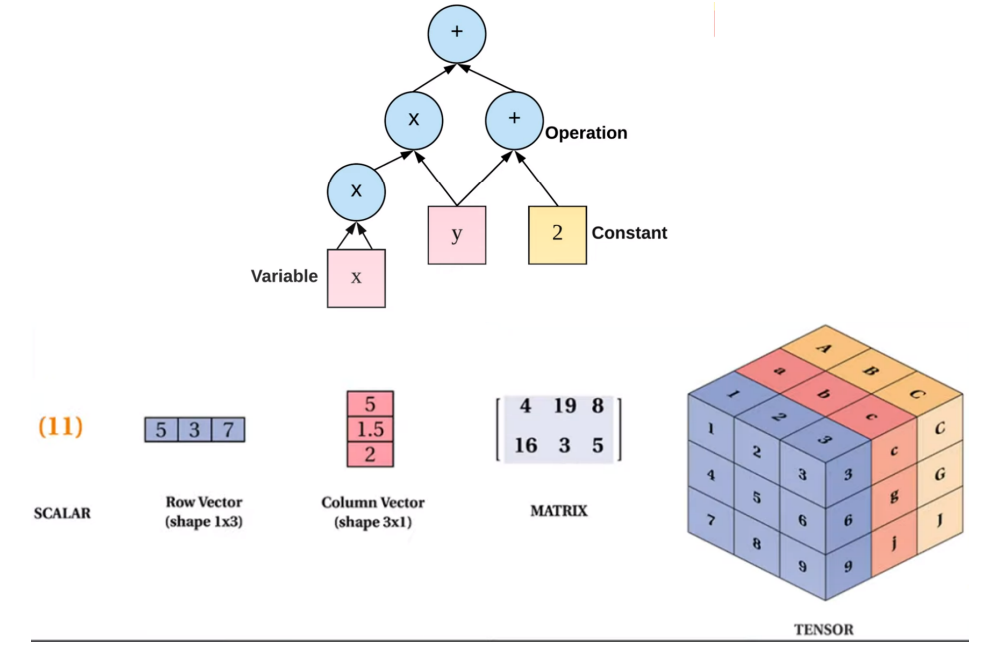
\includegraphics[width=5\textwidth, height=5cm, keepaspectratio]{tensor.PNG}
    \label{fig:enter-label}
\end{figure} 
\subsection{Raw Images / Aligned Images }
\subsubsection{Raw Image(Ham Görüntü)}
Bir sensör tarafından doğrudan yakalanan ve işlenmemiş olan orijinal görüntüdür.
Ham görüntü, genellikle sensör tarafından algılanan ışık yoğunluğu ve renk bilgisini içerir.
Ham görüntü, her pikselin sensör tarafından kaydedilen doğrudan değerlerini temsil eder. Bu nedenle, renk dengesi, pozlama ve diğer görüntü özellikleri genellikle işlenmemiştir.
\begin{figure}[h]
    \centering
    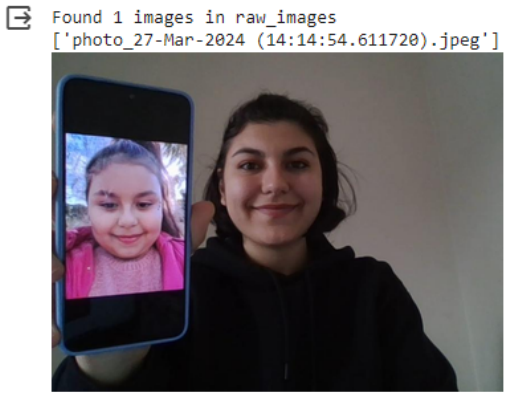
\includegraphics[width=5\textwidth, height=5cm, keepaspectratio]{raw.png}
    \includegraphics[width=5\textwidth, height=5cm, keepaspectratio]{rawleo.PNG}
    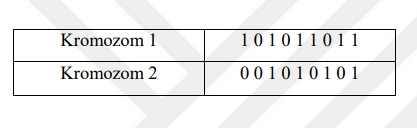
\includegraphics[width=5\textwidth, height=5cm, keepaspectratio]{iki.png}
    \caption{Raw Image Örneği }
    \label{fig:enter-label}
\end{figure} 
\newpage

\subsubsection{Aligned Image(Hizalanmış Görüntü)}
Hizalanmış görüntü, genellikle bir kaynak noktasına veya referans noktasına göre hizalanmış olan bir görüntüdür.
Hizalama işlemi, farklı görüntüler arasındaki konumsal farklılıkları veya dönüşümleri düzeltmek için yapılır.
\begin{figure}[h]
    \centering
    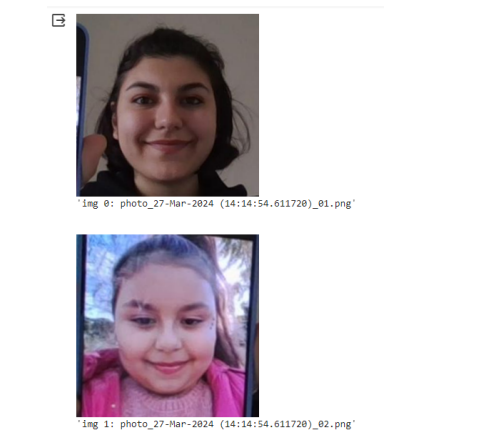
\includegraphics[width=5\textwidth, height=5cm, keepaspectratio]{aligned.PNG}
    \includegraphics[width=5\textwidth, height=5cm, keepaspectratio]{resim_2024-03-20_152545846.png}
    \includegraphics[width=5\textwidth, height=5cm, keepaspectratio]{uc.png}
    \caption{Aligned Image Örneği}
    \label{fig:enter-label}
\end{figure} \newpage
\subsection{Fast Version / Slow Version}
\subsubsection{Fast Version}

Hızlı sürüm, aynı işlevi yerine getiren ancak daha hızlı çalışan ve daha az kaynak tüketen bir versiyondur.
Genellikle daha az hesaplama yapılır veya daha az veri işlenirken kullanılır.
Hızlı sürüm, daha az doğruluk gerektiren veya daha basit problemleri çözmek için tercih edilebilir.
\subsubsection{Slow Version(Yavaş Sürüm)}

Yavaş sürüm, bir yazılım veya algoritmanın daha uzun sürede çalışan ve daha fazla kaynak tüketen bir versiyonudur.
Genellikle daha ayrıntılı hesaplamalar yapılır veya daha fazla veri işlenirken kullanılır.
Yavaş sürüm, daha doğru sonuçlar elde etmek veya daha karmaşık problemleri çözmek için tercih edilebilir.
\subsection{Optimizasyon Nedir ?}
Yapay sinir ağlarında uygulanan aşamalardan olan optimizasyon için öncelikle hata fonksiyonunun (loss function) tanımlanmasına ihtiyaç duyulmaktadır. Geleneksel ve modern yöntemlerde, optimizasyon demek, bir maliyet/kayıp fonksiyonunun belirli kısıtlara ve parametrelere tabi olarak en yüksek/düşük hale getirilmesi demektir.\cite{seyyarer2020derin}
\begin{figure}[h]
    \centering
    \includegraphics[width=5\textwidth, height=5cm, keepaspectratio]{resim_2024-03-27_161706406.png}
    \label{fig:enter-label}
\end{figure} 
Yapılan optimizasyon neticesinde bulunan minimum değerin, local minima değil, global minimaya götürmesi, optimizasyonun en önemli hedefidir. Eğitim setinde (training set) bulunan minimum değerler, en iyi sonuç bulunduğunu garanti etmez; optimizasyon, local minimaya düşmüş de olabilir. Bu yüzden hangi modelde hangi optimizasyonun uygulandığı önem kazanır.
\subsubsection{Momentum Algoritması}
Momentum, gradyan tabanlı optimizasyon algoritmalarında kullanılan bir tekniktir. Bu teknik, gradyanın yönüne ve büyüklüğüne bağlı olarak bir hız terimi ekleyerek güncellemeleri hızlandırır.

Örneğin, bir topun yokuş aşağı yuvarlanırken kazandığı momentumu düşünebilirsiniz. Her adımda, topun hızı, önceki adımlardaki hızı ve güncel gradyanın yönüne bağlı olarak belirlenir. Bu sayede, top daha hızlı aşağıya doğru hareket eder. Aynı şekilde, momentum terimi gradyan tabanlı optimizasyonlarda da benzer bir işlev görür.

Momentum, özellikle yerel minimumlardan kaçınmak ve daha hızlı yakınsamak için faydalı olabilir. Ancak, çok büyük bir momentum değeri modelin istenmeyen şekilde sıçramasına neden olabilir.
\subsubsection{RMSProp (Root Mean Square Propagation)Algoritması}
RMSProp, öğrenme oranını her parametre için ayrı ayrı ayarlayarak adaptif bir şekilde günceller. Bu sayede, nadir görülen özelliklere sahip parametrelerin daha hızlı güncellenmesi sağlanır.

RMSProp'un ana fikri, gradyanların değişim hızını izlemektir. Yani, büyük değişim hızına sahip parametrelerin öğrenme oranı küçültülürken, küçük değişim hızına sahip parametrelerin öğrenme oranı büyütülür. Bu, modelin daha dengeli bir şekilde güncellenmesini sağlar ve daha hızlı yakınsamasına yardımcı olabilir.

\subsubsection{ADAM (Adaptive Moment Estimation)Algoritması}
2015 yılında Toronto Üniversitesinde sunumu yapılan Adam optimizasyon algoritması; Momentum ve RMSprop algoritmalarını birleştirip kullanılan algoritmadır. Adam algoritması, son zamanlarda doğal dil işleme konularında geniş kabul görmüştür. Bu algoritma deep learning konularında çok kullanılmaktadır, çünkü iyi sonuçları hızlı şekilde vermektedir.

Moment ve RmsProb algoritmaları başlangıç değeri olarak sıfırdan başlamakta ve bu hız bakımında algoritmaları dezavantajlı duruma getirmekteydi. RMSProp ve Momentum algoritmalarında doğrudan türeve uygulanan yön düzeltmesi Adam algoritmasında önce iterasyon sayısına bağlı bir düzeltmeye tabi tutulur.
\[
\hat{M} = \frac{M}{1 - \beta_1^t}
\]


Bu düzeltme, momentum ve RMSProp algoritmalarının aksine Adam algoritmasının ilk iterasyondan itibaren etkin bir şekilde yakınsamaya başlamasını sağlar.\\

\textbf{ADAM Algoritmasının Avantajları} 

1-Algoritmanın uygulaması kolaydır.

2-Küçük hafıza gereksinimlerine ihtiyaç duyar.

3- Gürültülü veri setleri için uygundur.\cite{medium2023optimizasyon}\newpage
\begin{figure}[h]
  \centering
  \includegraphics[width=5cm, height=5cm, keepaspectratio]{ııııı.PNG}
  \caption{Şekil 1.4.3 \cite{seyyarer2020derin} makalesinden alınmıştır.}
  \label{fig:resim_etiketi}
\end{figure}


\subsection{Dnnlib Nedir?}
Dnnlib, NVIDIA'nın Derin Öğrenme Uygulamaları için Kütüphane (Deep Learning Applications Library) olarak bilinen bir kütüphanedir. Bu kütüphane, genellikle stilize edilmiş GAN modelleri gibi yenilikçi derin öğrenme tekniklerini uygulamak için kullanılır.

DNNLIB, TensorFlow ve PyTorch gibi derin öğrenme çerçevelerini destekler ve genellikle büyük ölçekli GANs eğitimleri için optimize edilmiştir. NVIDIA, özellikle StyleGAN gibi önde gelen GAN modellerini eğitmek için DNNLIB'i kullanmış ve bu modellerin eğitiminde önemli başarılar elde etmiştir.
\subsection{ResNet-18 Nedir ?}
ResNet, 2015 yılında Kaiming He, Xiangyu Zhang, Shaoqing Ren ve Jian Sun tarafından önemli ölçüde daha derin olan ağların eğitimini kolaylaştırmak için “Deep Residual Learning for Image Recognition” makalesinde tanıtılan belirli bir sinir ağı türüdür.\cite{youtube-video}\newline
\newline
\textbf{ResNet'in Başarıları }
\begin{enumerate}
    \item ImageNet veri setinde, VGG ağlarından daha derin, ancak yine de daha düşük karmaşıklığa sahip 152 katmana kadar derinliğe sahip artık ağların değerlendirilmesi sonucunda \%3,57 hata oranı ile ILSVRC 2015 sınıflandırma görevinde 1. oldu.
    \item Faster R-CNN’de VGG-16 katmanlarının ResNet-101 ile değiştirilmesiyle COCO nesne algılama veri kümesinde \%28 iyileşmeler gözlemlendi.
    \item ILSVRC ve COCO 2015 yarışmasında ImageNet Algılama, ImageNet yerelleştirme, COCO algılama ve COCO segmentasyonunda 1. oldu.
\end{enumerate}
Derin evrişimli sinir ağları ile birlikte görüntü sınıflandırması için bir dizi atılım olmuştur. Bu ağlarla beraber görüntü tanıma ve görüntü sınıflandırma gibi problemlerde son teknoloji sonuçlar elde edilmiştir. Böylece, yıllar içinde derin öğrenme mimarilerine giderek daha karmaşık görevleri çözmesi için daha fazla katman eklenerek daha derin bir hale getirilmiştir. Bu durum sınıflandırma ve tanıma görevlerinin performansını iyileştirmeye ve onları sağlam hale getirmeye yardımcı olmuştur.Katman eklemeye devam edersek  performans iyileşmesi olup olmadığı araştırılmıştır.20 katmanlı ağ ve 56 katmanlı ağ için eğitim ve test verilerindeki hata yüzdesini açıklayan bir grafik bulunmaktadır.\cite{he2016deep}
\begin{figure}[h]
    \centering
    \includegraphics[width=5\textwidth, height=5cm, keepaspectratio]{aaaa.PNG}
    \caption{Eğitim ve Test Verilerinde Hata Yüzdesini Açıklayan Grafik}
    \label{fig:enter-label}
\end{figure}\newline
\newline
\textbf{Grafikten Çıkarılan Sonuç:}
Sol taraftaki grafikte eğitim hatasını sağ taraftaki grafikte ise test hatasını görmekteyiz. Hem eğitim verisi hem de test verisi durumunda 56 katman için hata yüzdesinin 20 katmanlı bir ağdan daha fazla olduğunu görebiliriz. Bu, bir ağın üstüne daha fazla katman eklenmesiyle performansının düştüğünü gösterir. Çok derin sinir ağlarının eğitilmesi yakınsamayı engelleyen kaybolan/patlayan gradyanlar nedeniyle oldukça zordur. Teorik olarak derinliğini arttırdığımız ağda eğitim hatasının azalmasını bekleriz fakat gerçekte doğruluk doyar ve ardından hızla düşerek eğitim hatası artar. Bu ise aşırı uyum (overfitting) nedeniyle değil daha derin modellerin optimize edilmesinin kolay olmadığını gösteren bir bozulma(degredasyon)/optimizasyon probleminden dolayı olur.\\
\\
\textbf{Artık Blok (Residual Block)Nedir?}
\begin{figure}[h]
    \centering
    \includegraphics[width=5\textwidth, height=5cm, keepaspectratio]{artıkag.PNG}
    \caption{Artık Blok Grafiği}
    \label{fig:enter-label}
\end{figure}\newline
x katman girdisini toplama işlemine taşıyan düz çizgiye artık bağlantı (veya kısayol bağlantısı) denir. Kısayol bağlantıları bir veya daha fazla katmanı atlayanlardır. Artık bloklarla girdiler, katmanlar arasında kalan bağlantılar üzerinden daha hızlı yayılabilir.\cite{cilek2021resnet}


\subsection{Tensör Nedir ?}
Tensörler, sayılar, vektörler ve matrisler gibi verileri depolayan ve işleyen çok boyutlu dizilerdir. Tensörlerin boyut sayısı, "derece" olarak adlandırılır. Örneğin, bir sayı sıfırıncı dereceden bir tensördür, bir vektör birinci dereceden bir tensördür ve bir matris ikinci dereceden bir tensördür. Üçüncü dereceden bir tensör ise, bir matrisin katmanlardan oluşan bir küp şeklinde düşünülebilir.
Tensörler, verileri daha etkili bir şekilde temsil etmek ve işlemek için kullanılır. Özellikle yapay zeka ve makine öğrenimi gibi alanlarda, tensörler büyük miktarda veriyi depolamak ve çeşitli matematiksel işlemler yapmak için temel bir yapı taşıdır. Örneğin, bir görüntüyü renkli piksellerden oluşan üç boyutlu bir tensör olarak düşünebiliriz. Bir ses kaydını ise zaman ve frekans eksenleri üzerindeki ses dalgalarından oluşan iki boyutlu bir tensör olarak ifade edebiliriz.
\subsubsection{Tensörlerin Kullanım Alanları}
\textbf{Çok Boyutlu Veri Depolama:} Tensörler, nümerik verileri depolamak için kullanılır. Bu veriler, bir veya daha fazla boyutta düzenlenebilir ve saklanabilir. Örneğin, bir resmin piksel değerleri üç boyutlu bir tensörde saklanabilir: yükseklik, genişlik ve renk kanalları.

\textbf{Matematiksel İşlemler:} Tensörler, matematiksel işlemleri gerçekleştirmek için kullanılır. Toplama, çıkarma, çarpma, transpozisyon, matris çarpımı gibi işlemler tensörler üzerinde uygulanabilir.

\textbf{Derin Öğrenme ve Yapay Zeka:} Derin öğrenme ve yapay zeka alanlarında, tensörler verileri temsil etmek için yaygın olarak kullanılır. Sinir ağları ve diğer derin öğrenme modelleri, veri akışlarını ve hesaplamaları tensörler üzerinde gerçekleştirir.

\textbf{Model Eğitimi:} Tensörler, derin öğrenme modellerini eğitmek için kullanılır. Eğitim verileri, girdi verileri, hedef etiketler ve model parametreleri tensörler olarak temsil edilir ve eğitim algoritmaları bu tensörler üzerinde çalışır.

\textbf{Boyutlar:} Bir tensörün boyutlarına göre, farklı türlerde tensörler oluşturulabilir. Skaler (0D tensör), vektör (1D tensör), matris (2D tensör) ve daha yüksek boyutlu tensörler olabilir.

\textbf{Görüntü İşleme:} Görüntü verileri, tensörlerle temsil edilir. Renkli görüntüler genellikle üç boyutlu tensörler olarak temsil edilir: yükseklik, genişlik ve renk kanalları (RGB).

\textbf{Doğal Dil İşleme:} Metin verileri, tensörlerle temsil edilir. Kelime gömme teknikleri ve dil modelleri, metin verilerini tensörlere dönüştürerek analiz ve işlem yapar.

\textbf{Zaman Serileri Analizi:} Zaman serisi verileri, tensörlerle temsil edilebilir. Bu veriler üzerinde zaman serisi analizi ve öngörülebilirlik analizi gerçekleştirilebilir.
\subsection{PIL (Python Imaging Library)Nedir?}
PIL (Python Imaging Library), Python için bir görüntü işleme kütüphanesidir. PIL, görüntü dosyalarını açmak, işlemek ve kaydetmek için kullanılır. PIL ile, görüntülerin boyutunu değiştirebilir, döndürebilir, kesilebilir, birleştirilebilir ve filtreler uygulanabilir. PIL, JPEG, PNG, BMP, GIF ve diğer birçok yaygın görüntü formatını destekler. PIL görüntüsü, bir görüntüyü temsil etmek için kullanılan bir veri yapısıdır. Görüntünün piksellerini içerir ve farklı işlemler uygulamak için bir arayüz sağlar. Örneğin, bir PIL görüntüsünü gri tonlama dönüştürmek veya belirli bir boyuta yeniden boyutlandırmak gibi işlemler gerçekleştirilebilir.
\begin{figure}[h]
    \centering
    \includegraphics[width=3\textwidth, height=5cm, keepaspectratio]{pıllow.png}
    \label{fig:enter-label}
\end{figure}\newline
\begin{figure}[h]
    \centering
    \includegraphics[width=15\textwidth, height=8cm, keepaspectratio]{tablo.jpg}
    \caption{Projemizde Kullanılan Tensör ve PIL Örneği}
    \label{fig:enter-label}
\end{figure}
\newpage
\begin{figure}[h]
    \centering
    \includegraphics[width=8\textwidth, height=8cm, keepaspectratio]{xyz.PNG}
    \caption{Projemizde Kullanılan Tensör ve PIL Örneği 2}
    \label{fig:enter-label}
\end{figure} 
\subsection{ResNet Nedir ?}
ResNet, derin sinir ağlarının eğitilmesini kolaylaştırmak için geliştirilmiş bir evrişimli sinir ağı (convolutional neural network - CNN) modelidir. ResNet'in temel özelliği, ağın daha derin hale getirilmesine olanak tanıyan "skip connection" veya "shortcut connection" adı verilen bağlantıların eklenmesidir.

Bu bağlantılar, bir önceki katmandan sonra gelen katmanlara doğrudan bağlanarak, gradientlerin daha düzgün bir şekilde akmasını sağlar. Bu da daha derin ağların eğitimini kolaylaştırır ve ağın performansını artırır.

ResNet genellikle ImageNet veri kümesi üzerinde eğitilmiş ve çeşitli görsel tanıma görevlerinde başarılı bir şekilde kullanılmıştır. ResNet'in farklı versiyonları (örneğin, ResNet-50, ResNet-101, vb.) farklı derinliklere sahiptir ve farklı uygulamalara göre tercih edilebilir.
\begin{figure}[h]
    \centering
    \includegraphics[width=3\textwidth, height=3cm, keepaspectratio]{resnetkodda.png}
    \caption{Projede kullanılan ResNet kod parçası}
    \label{fig:enter-label}
\end{figure}
\begin{figure}[h]
    \centering
    \includegraphics[width=5\textwidth, height=5cm, keepaspectratio]{StyleGAN_proje1.png}
    \caption{ Projede kullanılan RGB ve ResNet Kullanımını Anlatan Çizim }
    \label{fig:enter-label}
\end{figure}
\newpage
\subsection{Latent Vektör Nedir ?}

Latent vektör, genellikle makine öğrenimi ve derin öğrenme alanlarında kullanılan bir terimdir. Özellikle, generatif modelleme gibi alanlarda sıkça karşımıza çıkar.

Bir generatif modelin öğrenme sürecinde, modelin girdisi olan verileri temsil etmek için kullanılan vektördür. Örneğin, GAN (Generative Adversarial Network) gibi bir modelde, latent vektör genellikle rastgele bir vektördür ve modelin öğrenme sürecinde bu vektör kullanılarak veri üretilir.

Latent vektör, genellikle modelin öğrenme sürecindeki gizli (latent) yapısını temsil eder. Bu vektör, genellikle bir önceki katmandan gelen çıktıların düzleştirilmesi veya kodlanması gibi işlemlerle elde edilir. Sonuç olarak, latent vektör, modelin öğrendiği temel özellikleri veya dağılımları içeren bir temsil olarak düşünülebilir.

Özellikle generatif modellerde, latent vektörün boyutu ve yapısı, üretilen verilerin kalitesi ve çeşitliliği üzerinde önemli bir etkiye sahip olabilir. Doğru bir latent uzay tasarımı, modelin daha iyi ve daha çeşitli veriler üretmesine yardımcı olabilir.
\begin{figure}[h]
    \centering
    \includegraphics[width=5\textwidth, height=5cm, keepaspectratio]{latent.png}
    \caption{latent vektör örneği 1 }
    \label{fig:enter-label}
\end{figure} 
\begin{figure}[h]
    \centering
    \includegraphics[width=5\textwidth, height=5cm, keepaspectratio]{panda.png}
    \caption{latent vektör örneği 2 }
    \label{fig:enter-label}
\end{figure} 

\begin{figure}[h]
    \centering
    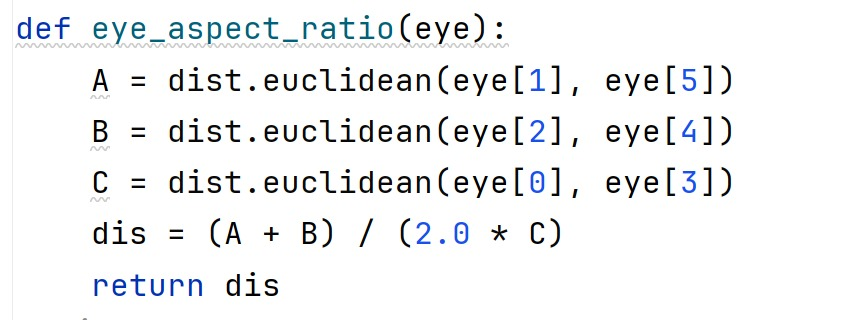
\includegraphics[width=5\textwidth, height=5cm, keepaspectratio]{kod.png}
    \caption{Projeden bir kod parçası }
    \label{fig:enter-label}
\end{figure} 
\subsection{ResNet-50 Nedir?}
ResNet-50'nin temel özelliği, önceki katmandan sonra gelen katmanlara doğrudan bağlantılar ekleyerek gradientlerin daha düzgün bir şekilde akmasını sağlayan "skip connection" veya "shortcut connection" adı verilen yapıyı kullanmasıdır. Bu yapı, ağın daha derin olmasını sağlayarak daha iyi öğrenme ve genelleme yetenekleri kazanmasını sağlar.

ResNet-50 modeli, genellikle evrişimli sinir ağlarıyla ilgili çeşitli görevlerde kullanılmaktadır, özellikle de transfer öğrenme uygulamalarında kullanılır. TensorFlow'da, önceden eğitilmiş ResNet-50 modelini kullanmak için\\
tf.keras.applications.ResNet50 gibi bir API bulunmaktadır. Bu API, ResNet-50 modelini ve ImageNet veri kümesinde eğitilmiş ağırlıklarını içerir, böylece bu modeli kolayca kullanabilir ve çeşitli görevler için uyarlanabilir.
\begin{figure}[h]
    \centering
    \includegraphics[width=6\textwidth, height=6cm, keepaspectratio]{RUYA1.PNG}
    \caption{Özellik vektörünü yazdıran bir kod çıktısı}
    \label{fig:enter-label}
\end{figure}
\begin{figure}[h]
    \centering
    \includegraphics[width=3\textwidth, height=4cm, keepaspectratio]{ekran1.png}
    \caption{Oluşturulan tahmini görüntü }
    \label{fig:enter-label}
\end{figure}
\newpage
\subsection{İki boyutlu evrişim (2D Convolution) Nedir?}

İki boyutlu evrişim (2D convolution), dijital görüntü işleme ve işaret işleme alanlarında sıkça kullanılan bir işlemdir. Temel olarak, bir girdi görüntüsü (veya işaret) ile bir evrişim çekirdeği (kernel) arasında bir matematiksel işlem yapmayı ifade eder.

Bu işlem, her bir pikselin (veya öğe) etrafında bir pencereyi (çekirdek) alır, bu pencereyi girdi görüntüsü üzerine yerleştirir, pencereyi ve çekirdeği eleman eleman çarparak toplar ve sonucu çıktı görüntüsüne (veya işarete) yazar. Bu işlem, girdi ile çekirdek arasında bir tür "çapraz-konvolüsyon" işlemidir.

2D evrişim genellikle görüntü işleme alanında kenar tespiti, görüntü filtreleme, özellik çıkarımı ve diğer birçok işlem için kullanılır. Örneğin, bir kenar tespit filtresi uygulamak için, kenarların görüntüdeki yoğunluk değişikliklerini vurgulayan bir çekirdek kullanılabilir.

İki boyutlu bilgiye uygulanacak olan filtrenin x ve y eksenine göre simetrisi alınır. Tüm değerler matriste eleman eleman çarpılır ve tüm değerlerin toplamı çıkış matrisinin ilgili elemanı olarak kaydedilir. Buna çapraz korelasyon ilişkisi de denir. Giriş verisi (örneğin; görüntü) tek kanallı iken bu işlem basitçe yapılabilmektedir. Ancak giriş verisi farklı formatlarda ve kanal sayısında olabilir.
\begin{figure}[h]
    \centering
    \includegraphics[width=5\textwidth, height=5cm, keepaspectratio]{raporson1.png}
    \caption{İki boyutlu evrişim işlemi gösterimi}
    \label{fig:enter-label}
\end{figure} 
\newpage
\subsection{RGB(Red,Green,Blue)Nedir?}

RGB (Red, Green, Blue), renkli görüntülerin temsil edilmesinde kullanılan bir renk modelidir. Bu modelde her piksel, kırmızı (Red), yeşil (Green) ve mavi (Blue) renk kanallarının bir kombinasyonuyla oluşturulur. Her bir renk kanalı 0 ile 255 arasında değer alabilir, bu da 8 bitlik bir renk derinliğine karşılık gelir.

Her bir RGB bileşeni, 0 ile 255 arasında bir sayıyla temsil edilir. Örneğin, (255, 0, 0) kırmızıyı, (0, 255, 0) yeşili ve (0, 0, 255) maviyi temsil eder. Bu renklerin her biri farklı yoğunluklarda karıştırılarak diğer renkler elde edilebilir. Örneğin, (255, 255, 255) beyazı, (0, 0, 0) siyahı temsil eder.

RGB modeli, bilgisayar ekranlarında ve dijital görüntüleme cihazlarında yaygın olarak kullanılmaktadır. Renkli görüntüler, her pikseldeki RGB değerlerinin birleştirilmesiyle oluşturulur ve her bir pikselin rengini belirler.

Renkli görüntüler, Kırmızı-Yeşil-Mavi (RGB) 3 kanaldan meydana gelmektedir. Bu koşulda da evrişim işlemi 3 kanal için yapılır. Çıkış işaretinin kanal sayısı da uygulanan filtre kanalı/sayısı ile eşit olarak hesaplanır.\cite{kizirak2018}
\newpage
\begin{figure}[h]
    \centering
    \includegraphics[width=8\textwidth, height=6cm, keepaspectratio]{MEDİUM.PNG}
    \caption{RGB'nin matris gösterimi\cite{kizirak2018}}
\end{figure}

\begin{figure}[h]
    \centering
    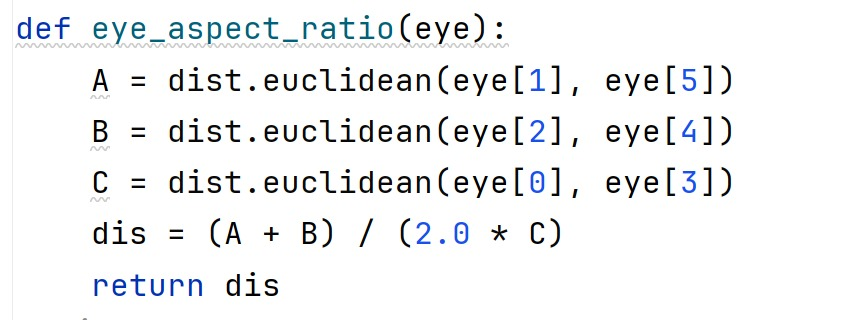
\includegraphics[width=8\textwidth, height=6cm, keepaspectratio]{kod.png}
    \caption{Bu kod ChatGPT tarafından yazılmıştır .\cite{chatgpt35}}
\end{figure}



\newpage
\printbibliography[title={Kaynakça}] 



\end{document}
